\documentclass[../main]{subfiles}

\graphicspath{{../figures/}}

\begin{document}

\section{屋外実験}
\label{sec:outdoor_experiment}
本研究では,実験室内での実験に加え,実際の石油精製施設内においても提案手法の性能を検証した.
本節では,実験環境の概要,実験手法,データの処理方法,得られた結果,そしてそれらに基づく考察について順に述べる.
\subsection{実験環境}
\label{subsec:vexp_ci_environment}
実験は,石油精製プラントの稼働エリアの一角で実施された.このエリアには,連続的に作動するポンプ類や,
定期的に圧力を放出するバルブ類が点在している.作業日当日もプラント全体が通常稼働中であり,背景騒音は実験室よりも格段に大きい環境であった.
また,足場や配管が立体的に入り組んでおり,音の反射や回折が多方向から生じやすく,音源の定位が困難となる複雑な空間が形成されていた.
\subsection{実験方法}
\label{subsec:vexp_ci_method}

まず,異常音源を一切配置しない状態で走行を複数回行い,正常運転時の騒音環境下におけるサンプルを収集した.
次に,異常を再現するための音源として,インパクトドライバと金属棒を定期的に打撃する装置を,プラント内の2箇所にそれぞれ配置し,
それらの位置を切り替えながら追加の走行を行った.
こうすることで,異なる位置で発生する異常音を検知できるかを評価すると同時に,
機器の連続作動音(インパクトドライバ)と間欠動作音(金属棒打撃)という異なる特性を持つ異常音を検知できるかを評価した.

\begin{table}[htbp]
  \centering
  \caption{各パスにおける各地点の異常音源}
  \label{tab:abnormal_sound_jp}
  \begin{tabular}{c|c|c}
  \hline
   & \textbf{地点A} & \textbf{地点B} \\ \hline
  \textbf{1回目} & 金属棒を打撃 & インパクトドライバ \\
  \textbf{2回目} & インパクトドライバ & 金属棒を打撃 \\ \hline
  \end{tabular}
\end{table}

\subsection{データの処理}
\label{subsec:vexp_ci_processing}
得られた音声信号は,実験室での評価時と同様に,まず48kHzのサンプリングレートで録音された後,前処理としてノイズ除去フィルタや正規化などの基本的な信号処理を施した.
続いて,短時間フーリエ変換を用いてパワースペクトルを抽出したのち,メルフィルタバンクを用いてスペクトログラムに変換し,
特徴量を抽出した.
なお,正常走行から得られたサンプルの一部をモデルの学習に用い,残りの正常サンプルと異常サンプルをテスト用として用いた.

\subsection{実験結果}
\label{subsec:vexp_ci_result}
屋外実験の結果,異常音源が設置されていない走行では,殆どのサンプルが正常音として正しく分類された.
一方,インパクトドライバや金属棒による定期的な打撃音が発生している走行では,これらの音源が存在する一付近のサンプルにおいて,
異常と判断される割合が顕著に増加した.
特に,インパクトドライバのような連続した衝撃音は,その周囲一体で一貫して異常判定を引き起こす傾向が見られたのに対し,
金属棒をたたく音は打撃が行われる時間帯のみ断続的に異常として認識された.

\begin{figure}[t]
  \centering
  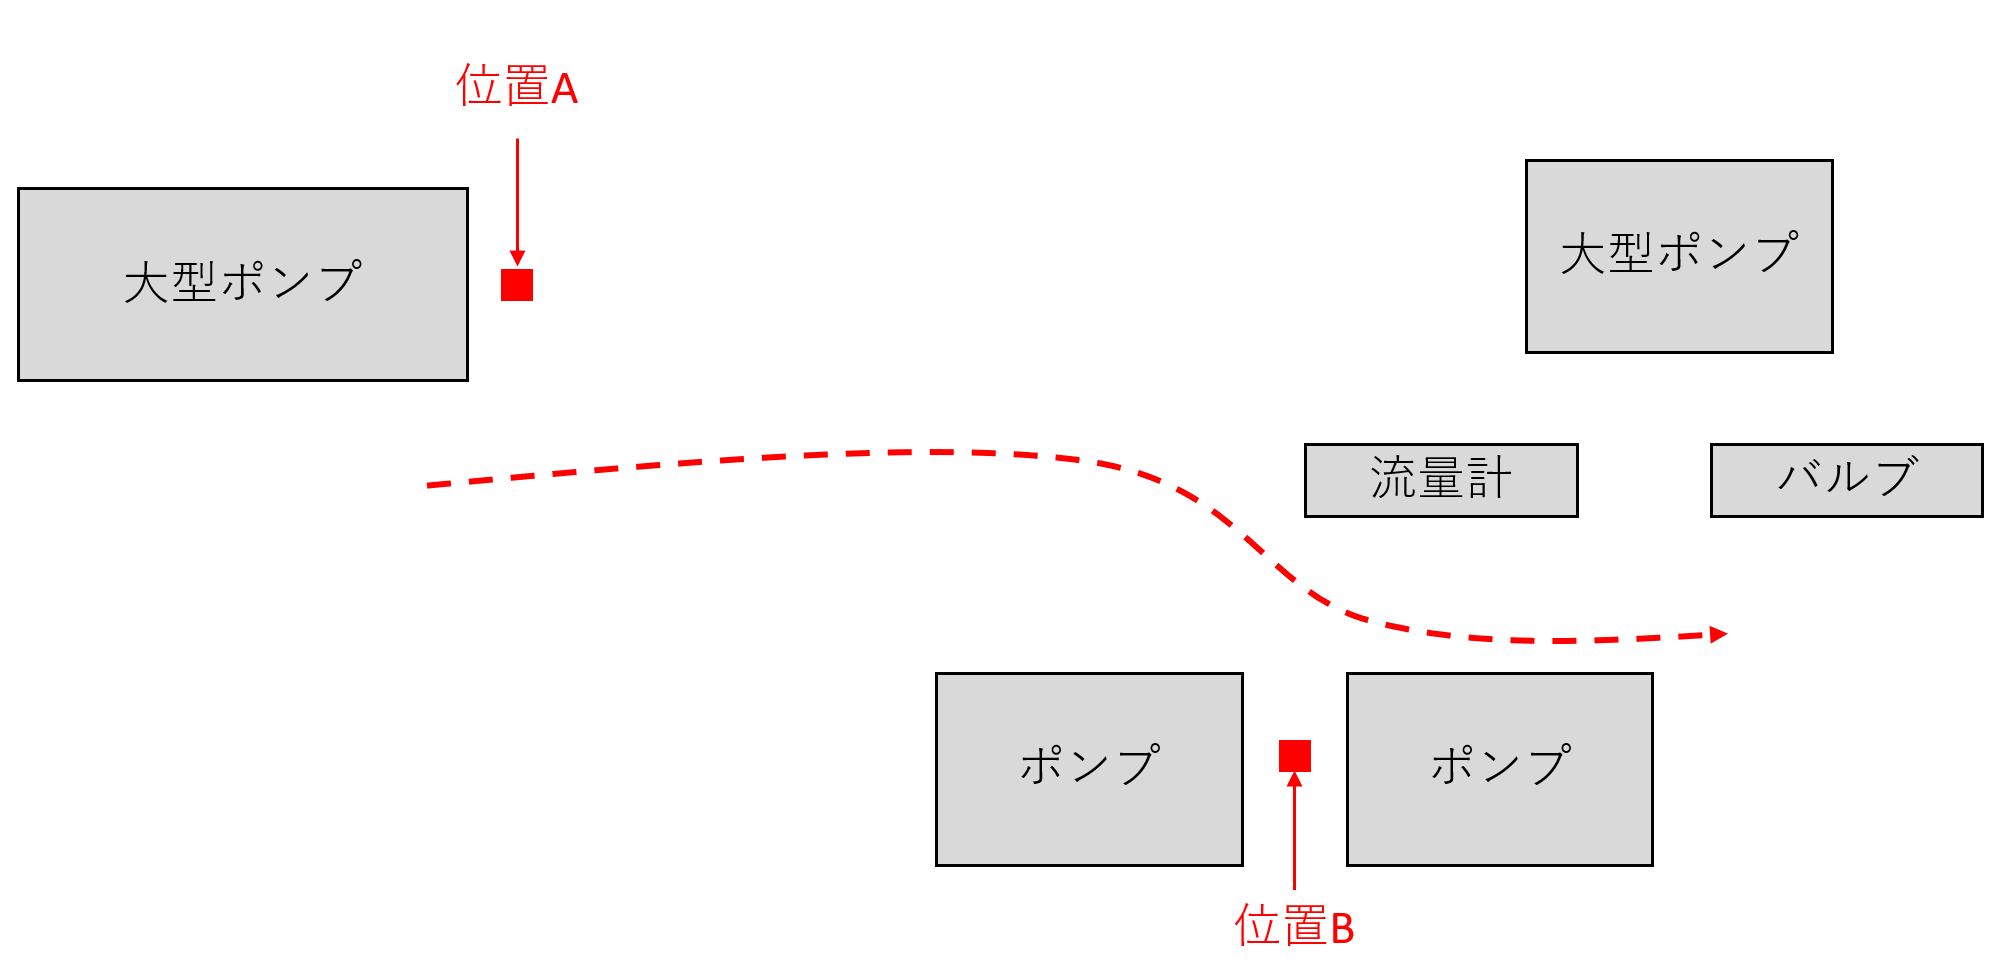
\includegraphics[keepaspectratio, width=1.0\linewidth]{chap4/field_environment.png}
  \caption{屋外実験における実験環境}
  \label{fig:field_environment}
\end{figure}

\begin{figure}[t]
  \centering
  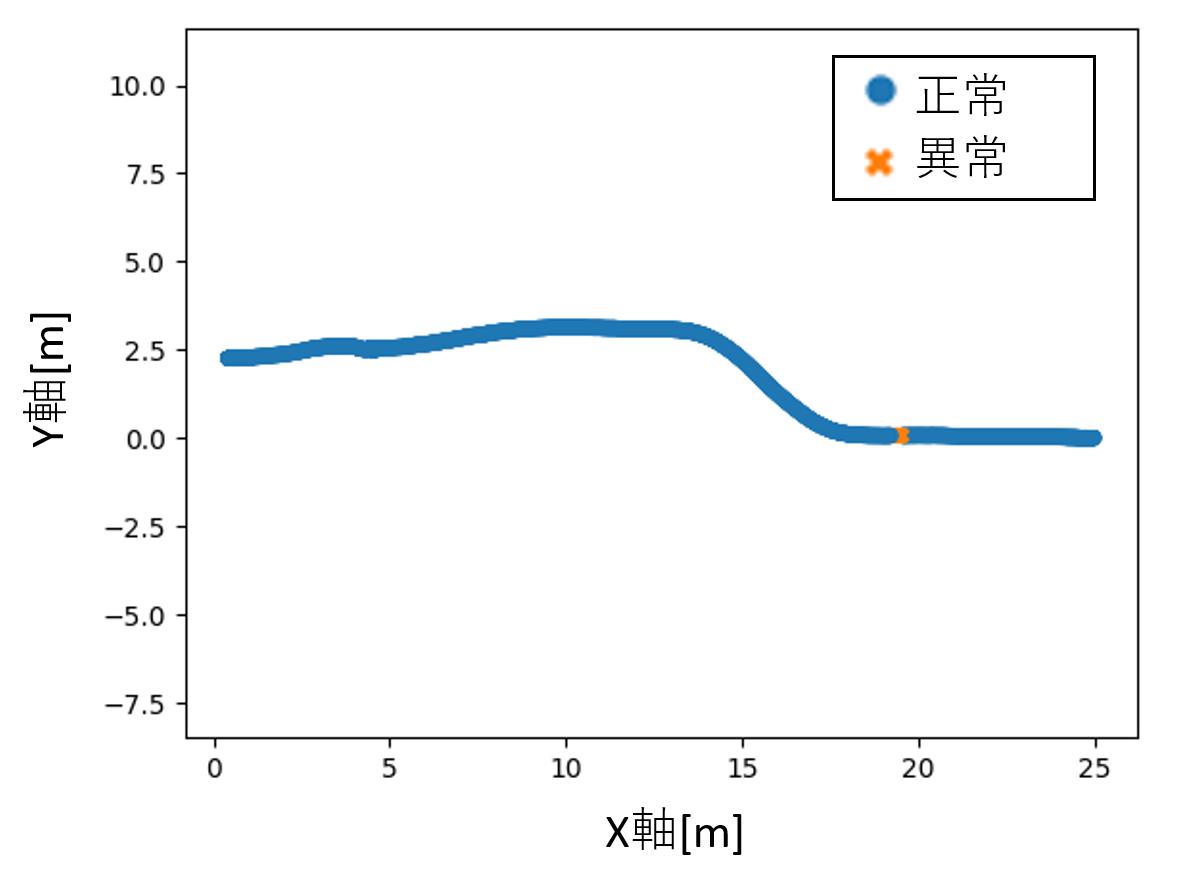
\includegraphics[keepaspectratio, width=0.7\linewidth]{chap4/field_normal.png}
  \caption{正常状態における異常検知結果}
  \label{fig:field_normal}
\end{figure}



\begin{figure}[t]
  \centering
  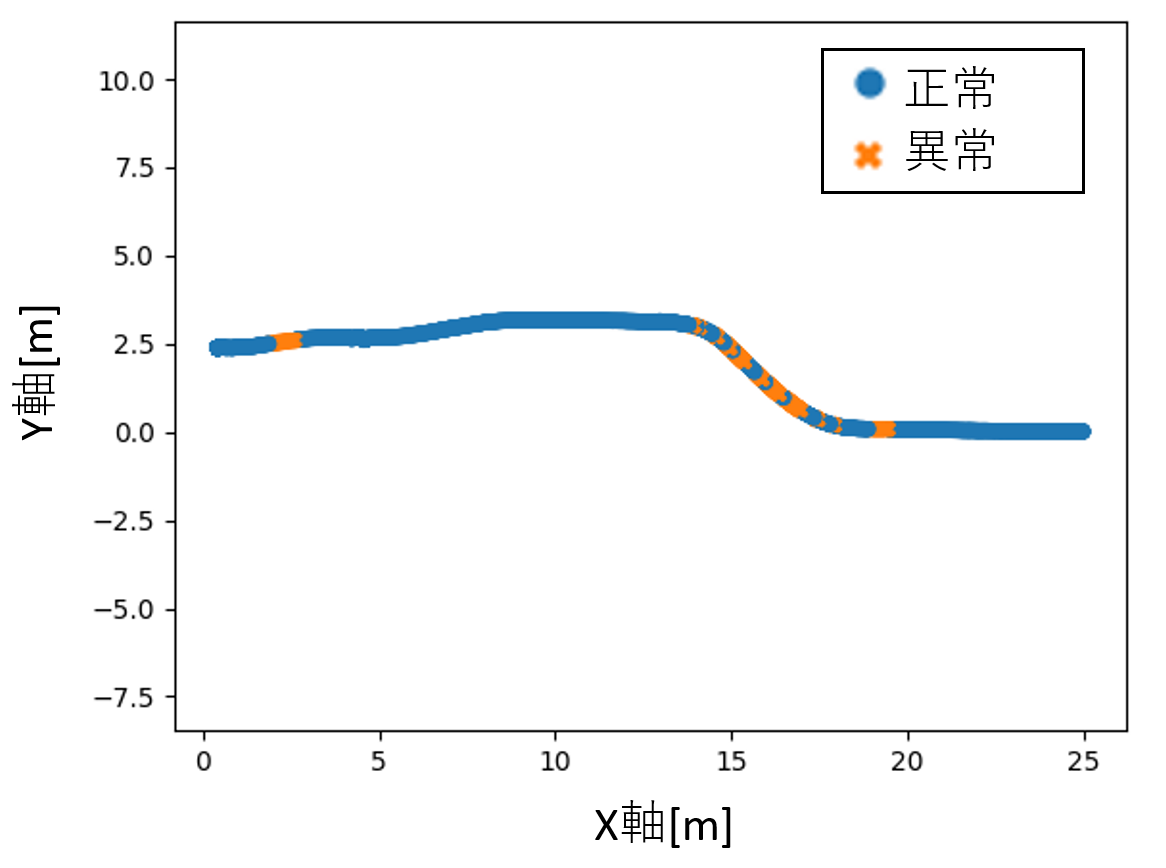
\includegraphics[keepaspectratio, width=0.7\linewidth]{chap4/field_abnormal1.png}
  \caption{異常状態における異常検知結果}
  \label{fig:field_abnormal1}
\end{figure}

\begin{figure}[t]
  \centering
  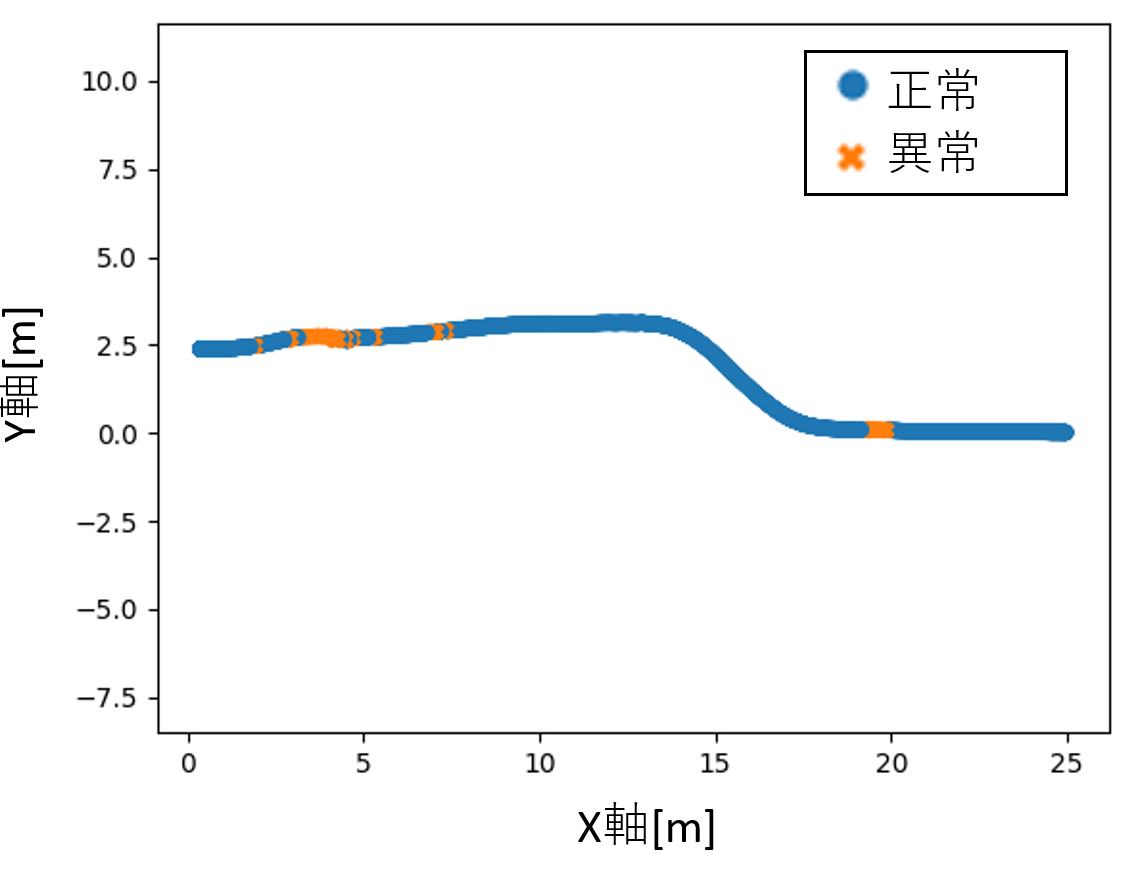
\includegraphics[keepaspectratio, width=0.7\linewidth]{chap4/field_abnormal.png}
  \caption{異常状態における異常検知結果}
  \label{fig:field_abnormal}
\end{figure}


\subsection{考察}

屋外実験においても,提案手法が異常音の検知に有効であることが示された.


\end{document}
